\documentclass[border=4pt]{standalone}
\usepackage{fontspec}
\usepackage{amsmath}
\usepackage{unicode-math}
\setmainfont{Latin Modern Roman}
\setmathfont{Latin Modern Math}
\usepackage{pgfplots}
\usepackage{pgfplotstable}
\pgfplotsset{compat=1.18}
\usepackage{tkz-euclide}
\usetikzlibrary{arrows.meta,calc,angles,quotes,patterns,3d,backgrounds}
\definecolor{ink}{HTML}{123428}
\definecolor{asy}{HTML}{475569}
\definecolor{mint}{HTML}{86e0bd}
\tikzset{asym/.style={asy, line width=0.9pt, dash pattern=on 5pt off 3.5pt},
         guide/.style={gray!70, line width=0.6pt, densely dotted},
         dot/.style={circle, inner sep=0pt, minimum size=5pt, draw=white, line width=0.5pt},
         odot/.style={circle, inner sep=0pt, minimum size=5.5pt, fill=white, line width=1pt},
         lab/.style={font=\footnotesize, inner sep=1.5pt, text=ink}}
\begin{document}
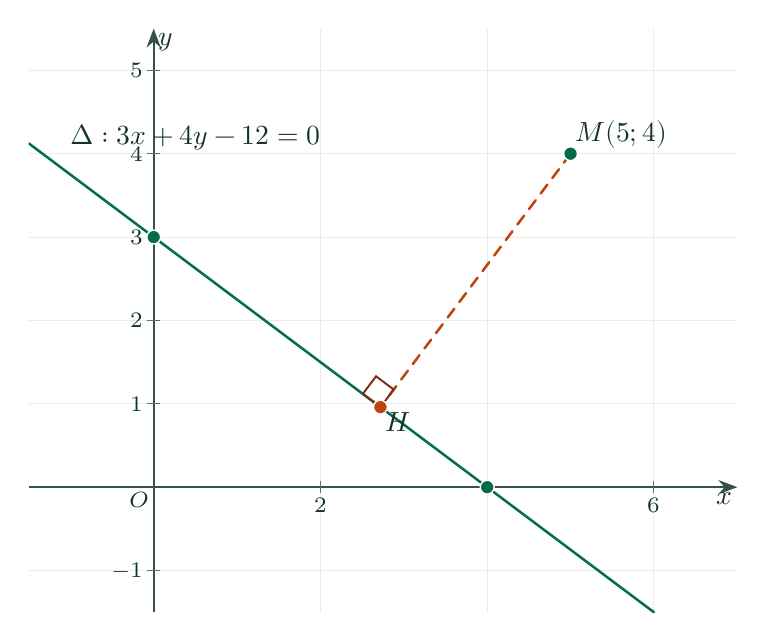
\begin{tikzpicture}[x=1.0588cm, y=1.0588cm]
\draw[gray!16, line width=0.4pt] (0,-1.5) -- (0,5.5) (2,-1.5) -- (2,5.5) (4,-1.5) -- (4,5.5) (6,-1.5) -- (6,5.5);
\draw[gray!16, line width=0.4pt] (-1.5,-1) -- (7,-1) (-1.5,0) -- (7,0) (-1.5,1) -- (7,1) (-1.5,2) -- (7,2) (-1.5,3) -- (7,3) (-1.5,4) -- (7,4) (-1.5,5) -- (7,5);
\draw[ink!85, line width=0.7pt, -{Stealth[length=2.4mm]}] (-1.5,0) -- (7,0) node[anchor=north east, lab, font=\normalsize] {$x$};
\draw[ink!85, line width=0.7pt, -{Stealth[length=2.4mm]}] (0,-1.5) -- (0,5.5) node[anchor=north west, lab, font=\normalsize] {$y$};
\draw[ink!70] (2,0.07555555555555556) -- (2,-0.07555555555555556) node[below, lab, font=\footnotesize] {$2$};
\draw[ink!70] (6,0.07555555555555556) -- (6,-0.07555555555555556) node[below, lab, font=\footnotesize] {$6$};
\draw[ink!70] (0.07555555555555556,-1) -- (-0.07555555555555556,-1) node[left, lab, font=\footnotesize] {$-1$};
\draw[ink!70] (0.07555555555555556,1) -- (-0.07555555555555556,1) node[left, lab, font=\footnotesize] {$1$};
\draw[ink!70] (0.07555555555555556,2) -- (-0.07555555555555556,2) node[left, lab, font=\footnotesize] {$2$};
\draw[ink!70] (0.07555555555555556,3) -- (-0.07555555555555556,3) node[left, lab, font=\footnotesize] {$3$};
\draw[ink!70] (0.07555555555555556,4) -- (-0.07555555555555556,4) node[left, lab, font=\footnotesize] {$4$};
\draw[ink!70] (0.07555555555555556,5) -- (-0.07555555555555556,5) node[left, lab, font=\footnotesize] {$5$};
\node[lab, anchor=north east] at (0,0) {$O$};
\tkzDefPoint(0,3){P}
\tkzDefPoint(4,0){Q}
\tkzDefPoint(-1.5,4.125){tmp1}
\tkzDefPoint(6,-1.5){tmp2}
\tkzDefPoint(5,4){M}
\tkzDefPoint(2.72,0.96){H}
\tkzDefPoint(0,3){tmp3}
\begin{scope}
\clip (-1.5,-1.5) rectangle (7,5.5);
\tkzDrawSegment[draw={rgb,255:red,4;green,107;blue,77}, line width=0.90pt](tmp1,tmp2)
\tkzDrawSegment[draw={rgb,255:red,194;green,65;blue,12}, line width=0.90pt, dash pattern=on 4pt off 3pt](M,H)
\end{scope}
\tkzMarkRightAngle[size=0.28, draw={rgb,255:red,124;green,45;blue,18}, line width=0.7pt](tmp3,H,M)
\node[dot, fill={rgb,255:red,4;green,107;blue,77}] at (P) {};
\node[dot, fill={rgb,255:red,4;green,107;blue,77}] at (Q) {};
\node[dot, fill={rgb,255:red,4;green,107;blue,77}] at (M) {};
\node[dot, fill={rgb,255:red,194;green,65;blue,12}] at (H) {};
\node[lab, font=\normalsize] at (0.5,4.2) {$\text{Δ}: 3x + 4y - 12 = 0$};
\node[lab, font=\normalsize, anchor=south west] at (5,4) {$M(5; 4)$};
\node[lab, font=\normalsize, anchor=north west] at (2.72,0.96) {$H$};
\end{tikzpicture}
\end{document}
